\section{Experimentation}
\label{sec:experimentation}

\noindent In order to assess the feasibility of our proposal we build a prototype called \emph{Topicalizer}, which implements the mechanisms described throughout this report, for the particular case of SOAP services. 

The implemented system receives as input a list of URIs from real WSDL interfaces available online. The system retrieves each WSDL and processes it by following the techniques outlined in sections \ref{subsub:soap} and \ref{subsub:Service-documentation-cleaning} and stores its relevant information into a service registry. In running this process, a stream of documents is generated, each one of them containing information related to a specific SOAP service operation. Then the stream of documents is categorized based on the document's content by applying the \emph{online LDA} algorithm as described in sections \ref{subsub:The-Latent-Dirichlet} and \ref{subsub:Application-of-LDA}. Such categorization arranges semantically-related documents into clusters which are defined by a weighted set of terms, that in turn become annotations on the operations that each document represents. The information gathered from the categorization process is specified in RDFS---conforming to the data model defined in section \ref{subsub:RDF-spec-of-KNOWEB}---and stored into an RDF triplestore.

The system architecture is depicted in Figure \ref{prototype-architecture}:

\begin{figure}
\begin{center}
 
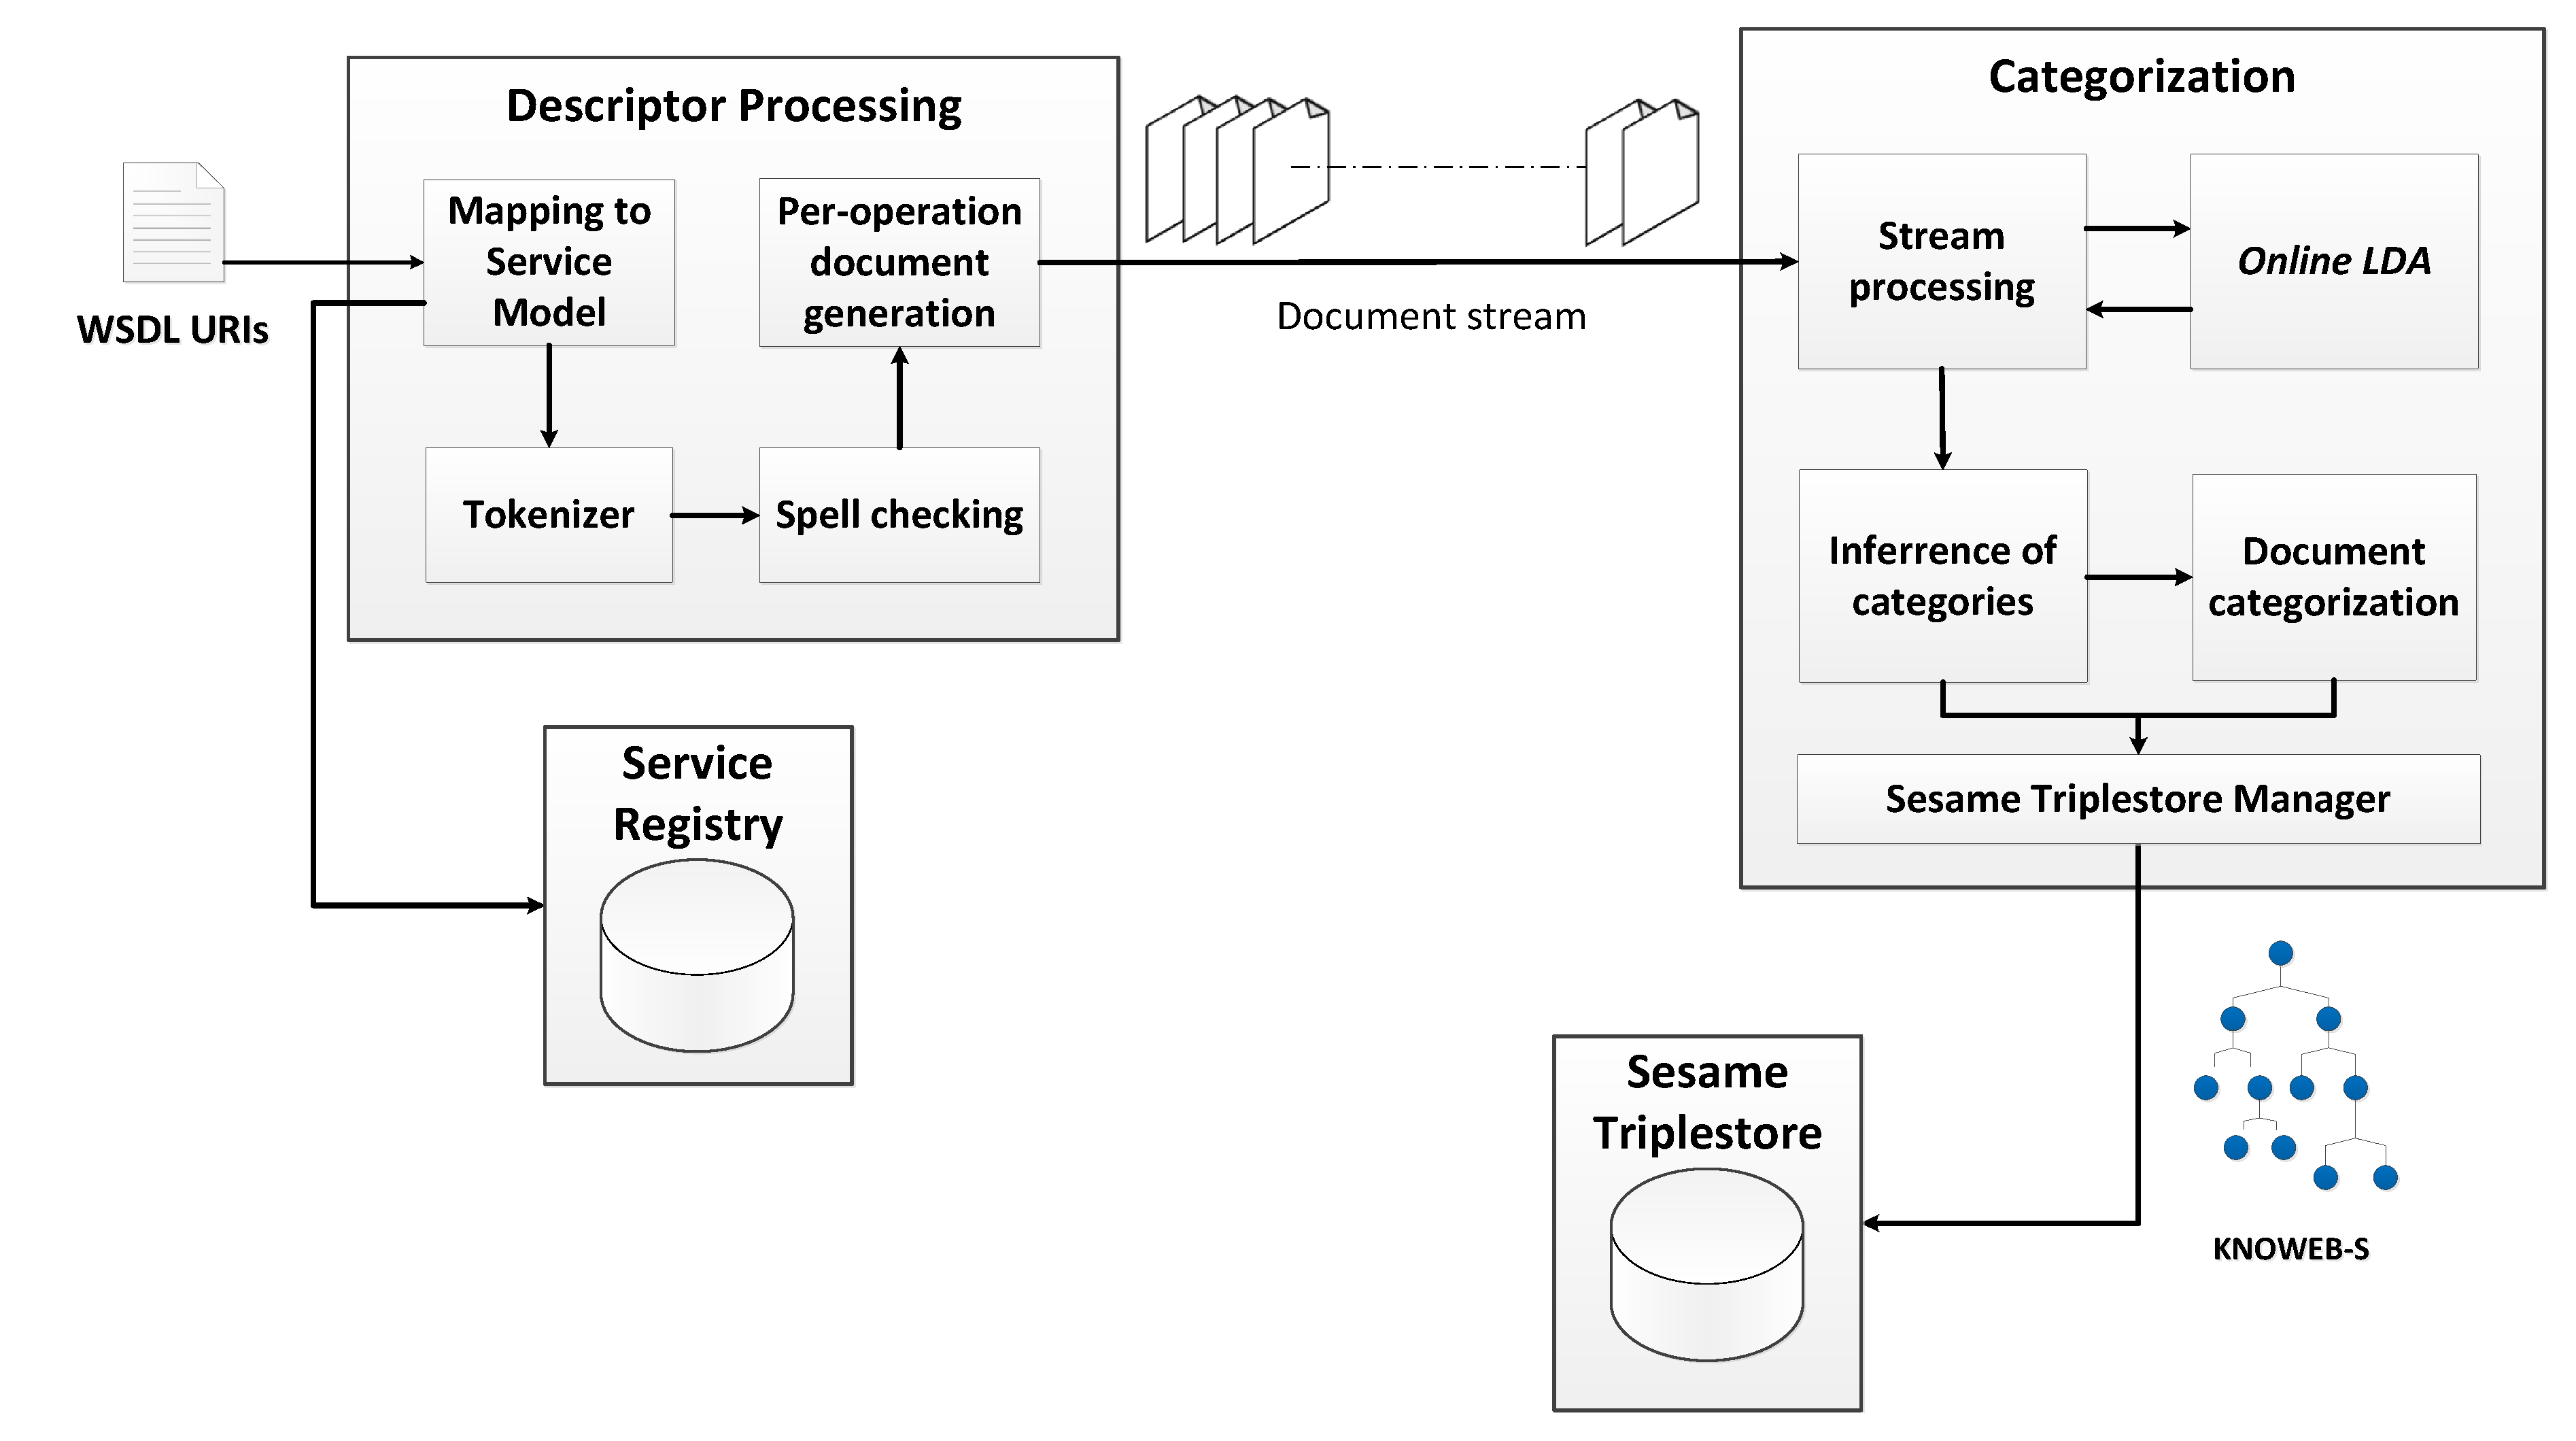
\includegraphics[scale=0.18]{images/prototype-architecture}

\caption{Architecture of Topicalizer.}
\label{prototype-architecture}
\end{center}
\end{figure}


Each one of the components comprising the architecture of Topicalizer are described below:
\begin{itemize}

\item \emph{Descriptor processing}: this module of the architecture is in charge of reading the list of WSDL URIs, accessing each descriptor via HTTP request, loading it into memory, mapping it into the SOAP service model defined in section \ref{subsub:soap} (see Figure \ref{wsdl-Simplified}) and storing the mapped information into a service registry. Once these initial procedures have been performed, this module applies tokenization and spell checking techniques---described in section \ref{subsub:Service-documentation-cleaning}---on the content of each descriptor and finally, for every operation of the processed descriptor it generates a document in plain text containing: (\emph{i}) the operation name, (\emph{ii}) its description in natural language, (\emph{iii}) the name of the service it belongs to, and (\emph{iv}) its input/output parameters. This module was implemented in Java, using its persistence API (JPA) and the \emph{EasyWSDL} library for WSDL manipulation \footnote{Available at: \href{http://
easywsdl.ow2.org/}{http://easywsdl.ow2.org/}}.

\item \emph{Service registry}: consists of a relational database, implemented in MySQL. The entity-relationship model of this database matches the service model described in section \ref{subsub:soap}. 

\item \emph{Categorization}: this component receives the stream of documents generated by the descriptor processing module, then splits it in small-sized batches and delivers them to the implementation of online LDA, which is based on an adaptation of an existing application developed by Matthew D. Hoffman, one of the authors of the mentioned algorithm \cite{Hoffman:2010}. Once the processing of the stream of documents is completed, the derived results are interpreted for establishing the set of terms that compose each category---task performed by the \emph{inference of categories }sub-module---as well as the group of documents included in each one of them---which is defined by the \emph{document categorization} sub-module. The derived arrangement of categories, documents and terms, is mapped into the KNOWEB-S data model and stored into a RDF triplestore provided by the \emph{Sesame} openRDF framework \footnote{Available at: \href{http://www.openrdf.org/index.jsp}{http://www.openrdf.org/index.jsp}}. This 
component of the architecture was developed in Python, using the \emph{numpy}, \emph{urllib2} and \emph{httplib2} libraries.

\item \emph{Sesame Triplestore}: It is an HTTP repository for RDF triples, hosted in an Apache Tomcat web server. This repository stores the KNOWEB-S taxonomy generated by the previous Categorization component. Sesame allows the retrieval and manipulation of the information encoded in KNOWEB-S by using SPARQL queries.
\end{itemize}

The whole prototype is executed by using a bash script, which receives as input the path of a text file containing the list of WSDL URIs. The prototype also generates two documents in \emph{csv} format for specifying: (1) the terms that define each of the identified categories along with their associated relevance value, and (2) the per-document category proportions for each of the processed documents (i.e. SOAP service operations).  
A description of the source code structure of the prototype is available at \href{https://github.com/LeandroOrdonez/Topicalizer}{https://github.com/LeandroOrdonez/Topicalizer}.

For evaluating ou proposal, we have developed a web application \footnote{\textit{TopicalizerBrowser}, available at \href{http://leandrocloud.cloudapp.net:8080/TopicalizerBrowser}{http://leandrocloud.cloudapp.net:8080/TopicalizerBrowser}} (Figure \ref{topicalizer-browser}) intended for human evaluators to visualize and browse through the structure of categories (topics) that pervade a corpus of 200 SOAP service descriptors (which add up to 1328 operations) extracted from the research dataset by Zhang et al. \cite{Zhang:2010}. We asked the evaluators to estimate the coherence of the categorization as well as the relevance of the annotations that our prototype assigns to each individual operation. The procedure that each evaluator followed consist of two steps:

\begin{enumerate}
 \item When assessing a \textit{category}, the evaluator has to assign a name to it, based on its distribution over terms and the operations it contains. Whenever there is no obvious name for a particular category according to the evaluator's judgment, the assigned name is set to ``\textit{NA}'' (i.e. \textit{Not Available})
 \item When assessing an \textit{operation} the evaluator must estimate the relevance of the annotations that the prototype has assigned to it, by approving or disapproving them, and adding new terms that he/she considers the prototype has missed. Figure \ref{evaluated-operation} shows the outcome of performing this step on one web service operation.
\end{enumerate}

We had three evaluators taking part on this process. They went through this procedure on 11 randomly selected categories out of the 40 available, performing the evaluation of 155 operations (that is 15 operations per category).


\begin{figure}[H]
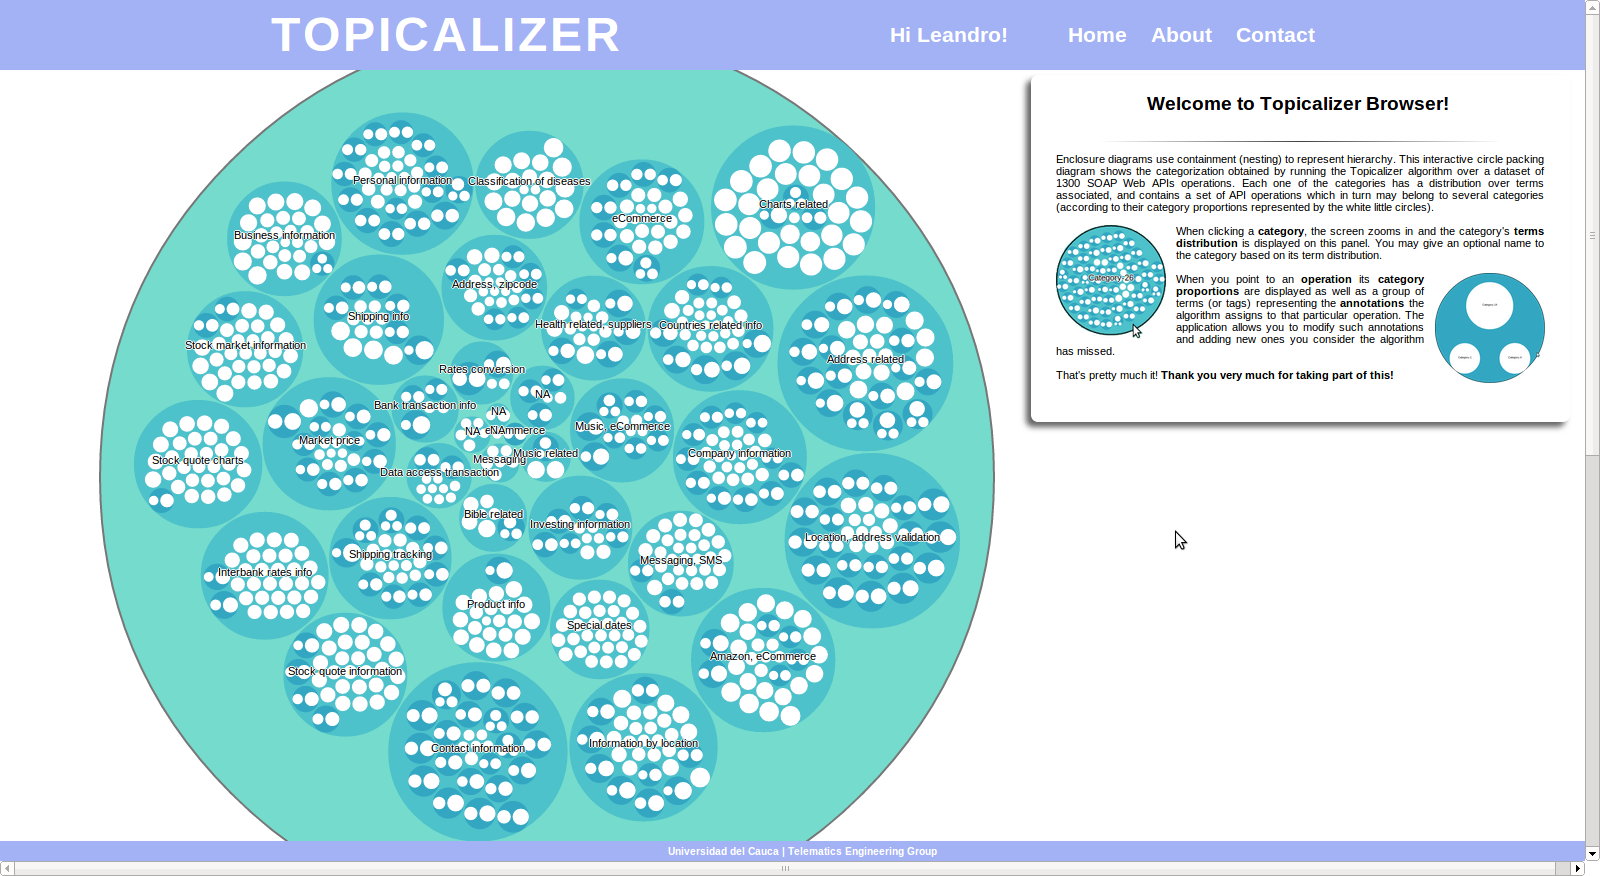
\includegraphics[scale=0.215]{images/TopicalizerBrowser}

\caption{Topicalizer Browser Application}
\label{topicalizer-browser}

\end{figure}

\begin{figure}[H]
\begin{center}
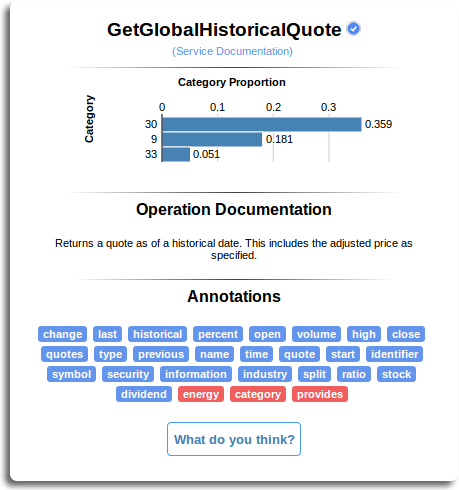
\includegraphics[scale=0.40]{images/EvaluatedOperation}
\caption{Example of a Web service operation annotated by Topicalizer. Blue tags represents the accepted annotations, while red ones are rejected annotations according to the judgment of the evaluator.}
\label{evaluated-operation} 
\end{center}
\end{figure}

Based on the results gathered from this evaluation procedure, we estimate the performance of our proposal by taking three measurements on each of the operations reviewed by the human evaluators: \textit{Precision (P)}, \textit{Recall (R)} and the \textit{Balanced F-measure ($F_1$)}. All three measurements were estimated on each evaluated operation according to the following expressions:

\begin{equation}
P_{op}=\frac{1}{\left|E\right|}\sum_{e=0}^{\left|E\right|}{\displaystyle {\textstyle {\displaystyle \frac{\left|AA_{e}\right|}{\left|RA_{e}\right|+\left|AA_{e}\right|}}}}\label{eq:3}
\end{equation}

\begin{equation}
R_{op}=\frac{1}{\left|E\right|}\sum_{e=0}^{\left|E\right|}{\displaystyle {\textstyle {\displaystyle \frac{\left|AA_{e}\right|}{\left|MA_{e}\right|+\left|AA_{e}\right|}}}}\label{eq:4}
\end{equation}

\begin{equation}
F_{1_{op}}={\displaystyle {\textstyle {\displaystyle \frac{2P_{op}R_{op}}{P_{op}+R_{op}}}}}\label{eq:5}
\end{equation}

where $AA_{e}$, $RA_{e}$ and $MA_{e}$ refer to the sets of \textit{accepted}, \textit{rejected}, and \textit{manual} (non-existent) annotations for evaluator $e$ respectively, while $\left|E\right|$ represents the number of evaluators.

When computing the overall precision, recall and F-measure by summing over all the evaluated operations $op$, the average value of each measurement were respectively 81.48\%, 90.48\% and 85.45\%, outperforming similar approaches, like the one proposed by Falleri et al. in \cite{Falleri:2010}. Figure \ref{p-vs-r} provides a detailed view of the results in terms of the precision and recall of individual operations in the dataset. This graph evidences the capability of our proposal for assigning a \textit{comprehesive} (high recall) set of \textit{relevant} (high precision) annotations to each operation in the dataset since all datapoints lie in the upper right corner of the precision--recall chart.

\begin{figure}[H]
\begin{center}
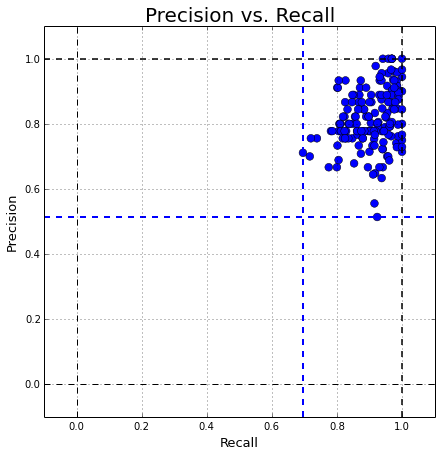
\includegraphics[scale=0.52]{images/PvsR}
\caption{\textit{Precision} vs \textit{Recall} for individual operations in the dataset}
\label{p-vs-r} 
\end{center}
\end{figure}

Figure \ref{prf-vs-c} depicts the average value of precision, recall and F-measure per category. Additionaly this chart shows the set of terms defining each one of the evaluated categories. According to this graph, our system is able to identify semantic related tokens out of the content of web services descriptors, while properly classify service operations within the categories each set of terms defines, with an F-measure ranging from 79.24\% (category 3) to 95\% (category 8).

The results we got from the performance evaluation evidences the feasibility of our approach for classifying and annotating web services supported on probabilistic topic models. It is worth noting that, even though the evaluation was performed on SOAP services, the proposed mechanism would be also suitable for XML-RPC and REST-like web services as long as their documentation is available in a semi-structured format (e.g. HTML documents) so that it can be handled according to the process outlined in section \ref{subsubsec:rpc-rest}.

\begin{sidewaysfigure}
\begin{figure}[H]
\begin{center}
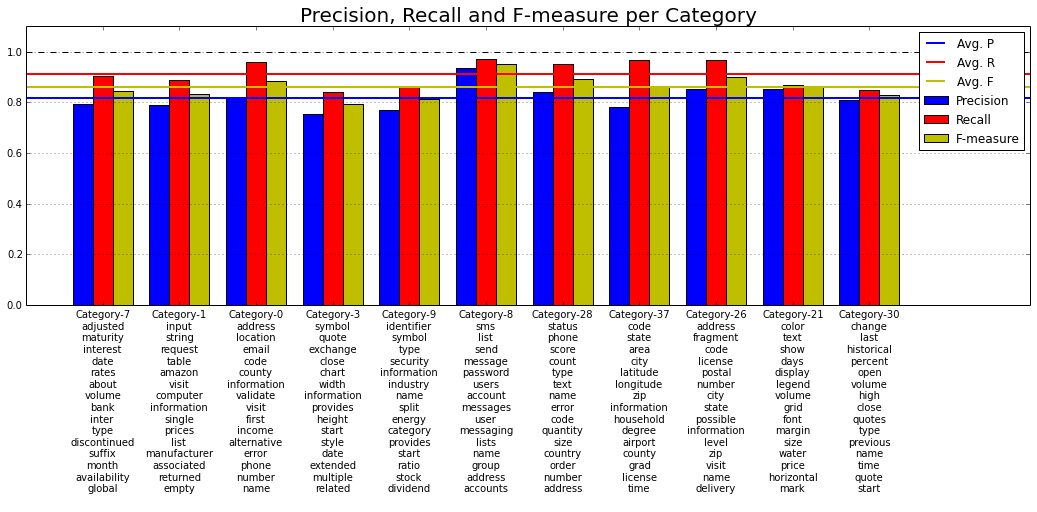
\includegraphics[scale=0.52]{images/PRFvsC}
\caption{\textit{Precision}, \textit{Recall} and \textit{F-measure} per Category. Note that the list of terms defining each category is placed under the Category IDs.}
\label{prf-vs-c} 
\end{center}
\end{figure}
\end{sidewaysfigure}



